%%%%% Design %%%%%
\section{Design} 
\subsection{Structural Design} % Done by Jiachen Wu
The novel Continuous Six-degree-of-freedom Manipulator introduced in this paper, which corresponds to the scheme design 
shown in Figure \ref{fig:fishboneCR_2023bio}, belongs to the class of bio-inspired continuum robots \cite{fishboneCR}. 
In the design process, a nylon cable drive mechanism is emloyed as a substitute for the complex musculature of fish, 
enabling it to maintain stability while undergoing deformation movements, thus achieving effective deformation motion 
and controllability. As depicted in Figure \ref{fig:main_components}, the rigid cross-shaped sheets is utilized to mimic 
the spine and ribs, uniformly arranging these sheets on a rubber pure soft sleeve to replace the spinal joints.
\begin{figure}[H] %[H] "corresponds to start the figure Here" 
    \centering %alignment can be flushleft or flushright
    \captionsetup{labelsep=colon}
    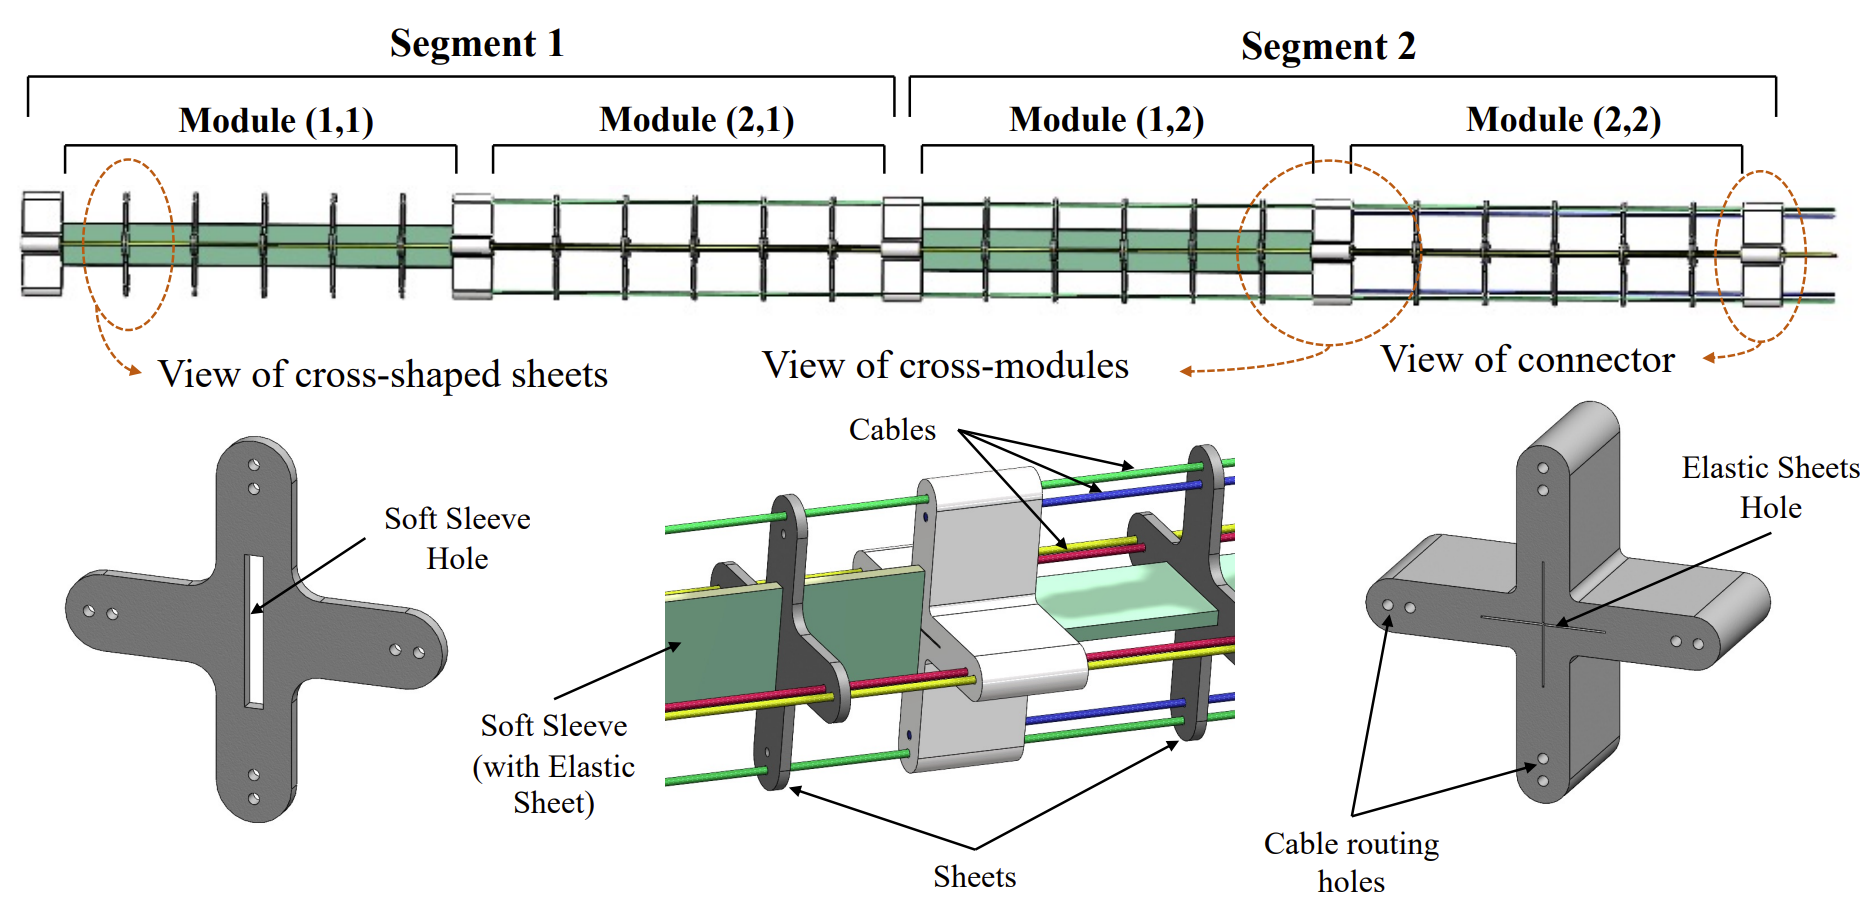
\includegraphics[width=1.0\textwidth]{Image/Design/main_component_of_manipulator.png} 
    \caption[The main components of the proposed manipulator and cables arrangement]
    {\centering \textbf{The main components of the proposed manipulator and cables arrangement.}}
    \label{fig:main_components}
\end{figure}
\subsection{Designation and Parameter Definition of Manipulator} % Done by Jiachen Wu, Zehao Ye do the table part
The manipulator is composed of four identical modules, each of which can be independently controlled to bend within a 
two-dimensional space. Each module consists of an elastic sheet and five uniformly arranged cross-shaped sheets, where 
the rubber pure soft sleeve outside the elastic sheet is interference-fitted with the cross-shaped sheets. The connector 
end of each module features two symmetrically arranged inextensible cables that pass through the cross-shaped sheets and 
are anchored to the connector, driving the end of each manipulator module. By applying tension to one of these cables, 
the elastic sheet can be deflected, thereby achieving a single degree of freedom planar motion at the end of the 
manipulator module. Since the elastic sheets of the modules are transversely mounted, the deflection of two or more 
sheets simultaneously allows for spatial motion at the end of the manipulator, as shown in Figure \ref{fig:main_components}. 
Overall, the proposed manipulator comprises two segments, each maintaining a constant length of 675mm and a weight of 
88 grams. Each module contains five cross-shaped sheets with a circumferential radius of 20mm and a thickness of 1.5mm. 
Both the head and the tail of each segment are connected by connectors, which have the same circumferential radius as 
the cross-shaped sheet and a thickness of 15mm. \\
The definition of manipulator parameters is presented in Table \ref{tab:parameter_name}. The subsequent sections 
will adhere to the corresponding naming conventions.
\begin{center}
    \small
    \begin{longtable}{l l l }
    \caption{The Parameters of Manipulators.} \label{tab:parameter_name} \\
    \hline \multicolumn{1}{l}{\textbf{Paramter}} & 
    \multicolumn{1}{l}{\textbf{Definition}} & 
    \multicolumn{1}{l}{\textbf{Value (mm)}} \\ \hline 
    \endfirsthead
    \multicolumn{3}{c}%
    {{\bfseries \tablename\ \thetable{} -- continued from previous page}} \\
    \hline \multicolumn{1}{l}{\textbf{Paramter}} & 
    \multicolumn{1}{l}{\textbf{Definition}} & 
    \multicolumn{1}{l}{\textbf{Value (mm)}} \\ \hline 
    \endhead
    \hline \multicolumn{3}{|r|}{{Continued on next page}} \\ \hline
    \endfoot
    \hline \hline
    \endlastfoot
    % table context
    $Sr_i$       & the length of elastic sheet in Module i      & $Sr_{1,2,3,4} = 150$ \\ 
    $d_i$        & the thickness of the cross-shaped connector  & $d_{1,2,3,4,5} = 15$ \\ 
    $N$          & the number of cross-shaped sheet in a module & $N = 0 \text{ \raisebox{-0.7ex}{\textasciitilde} } 15$ \\ 
    $r_i$        & the distance between the centroid of         & $r_{1,2} = 17.5$ \\
                 & connector and cable routing hole             & $r_{3,4} = 15$ \\
    $\Delta S_i$ & the change rate of cable, cable$_{2i-1}$ and & \\
                 & cable $_{2i}$ corresponds to Module i        & \\
    \hline
    % \multirow{2}{*}{3D cartesian/gantry manipulator} & PPP & 3 & 1   \\
    % & & & \\ \hline
    \end{longtable}
\end{center}
\subsection{Material Selection}
The fabrication of the Continuous Six-Degree-of-Freedom Manipulator primarily employs the following methods: Shape 
Deposition Manufacturing (SDM)\cite{fast_and_robust}, Casting\cite{recipe2015,high_force}, and Multi-material 3D 
Printing Technologies\cite{evolution2016,3Dprint_design}. By integrating SDM with Casting techniques, it is possible 
to utilize rigid, flexible, and soft materials, and integrate components such as sensors and circuits into the structure, 
which is particularly crucial for the integrated manufacturing of sensors and actuators. On the other hand, Multi-material 
3D Printing technology supports the unified manufacturing of soft and hard materials, enabling the creation of structures 
with more complex geometries and adjustable material hardness according to specific requirements. This approach results 
in structures that are not only more scientifically arranged and exhibit a more rational combination of rigidity and 
flexibility but also possess higher stability and superior performance. Moreover, Multi-material 3D Printing enhances 
manufacturing efficiency. Given these advantages, 3D Printing technology emerges as the preferred method for constructing 
continuum robots. \\
The materials for the cross-shaped sheets and connectors can be fabricated in an integrated manner using Multi-material 
3D Printers, which avoids the impact of imperfect assembly on deformation and achieves a compact design. The material 
chosen simulates engineering plastics (Mainly digital material with a Poisson's ratio of 0.394, a modulus of elasticity 
of 2.2 GPa and a Young's modulus of 2.5 GPa). The soft sleeve material is made of silicone rubber, characterized by a 
Poisson's ratio of 0.47. Furthermore, a 65Mn alloy steel (with a Poisson's ratio of 0.244 and a Young's modulus of 0.2 
GPa) elastic sheet (flexible) embedded within the soft sleeve forms a bio-inspired sheath, creating a bio-inspired 
fishbone structural unit. This structural unit is a hybrid of rigidity, flexibility, and softness, not only exhibiting 
excellent constant curvature characteristics but also higher structural stability. The bio-inspired fishbone unit also 
provides a constraint mechanism for the synchronous bending of the driving cables, effectively reducing the impact of 
external mechanical collisions on the cables \cite{fishboneCR}. Therefore, this unique structural design is a key 
foundation for achieving high-precision modelling of continuum robots. \\
In this design, the elastic sheet is combined with the connector by embedding it into a 0.3mm wide slot on the connector 
and utilizing an interference fit, a method that eliminates the need for additional fasteners and ensures the structural 
integrity of the continuum robot during standard operations. Nonetheless, to prevent the robot from separating under 
extreme overload conditions, special fixing holes were designed on both the elastic sheet and the connector. The 
installation of screws through these holes enhances the robustness of the continuum robot in harsh environments. 
Leveraging the modular design characteristic of the continuum robot, it can be constructed by serially connecting 
multiple similar motion modules. The example demonstrated in this study is comprised of two such motion modules, as 
shown in Figure \ref{fig:main_components}, whereby altering the length of the driving cables enables the continuum 
robot to achieve multi-degree of freedom movements. \\
Figure \ref{fig:main_components} illustrates the cable configuration scheme proposed for the continuum robot in this 
paper. Each bio-inspired fishbone structural unit is actuated by two symmetrically arranged cables, which traverse 
through the guide holes of the connectors and cross-shaped sheets, with each module being controlled by two motors, 
totaling eight motors. The guide holes in the cross-shaped sheets ensure that the cables maintain an arc shape within 
their bending region. In the actual design process, the maximum number of cross-shaped sheets is determined by the 
maximum bending angle preset for the bio-inspired fishbone unit. Through simulation analysis, we have concluded that 
the bending performance of the elastic sheet is optimal when the bending angle reaches 73°. \\
The design proposal offers the following advantages: \\
\begin{itemize}
    \item Lightweight: Utilizing cross-shaped sheets results in a lighter weight compared to traditional cylindrical manipulators.
    \item Stable Deformation Motion: The deformation motion is stable, offering an improvement over traditional cylindrical manipulator.
    \item Rigidity: The adoption of a stacked skeleton structure effectively eliminates bending deformation.
    \item Energy Consumption \cite{bio_noval_method}: The proposed robot design facilitates a reduction in the energy required to achieve spatial movement; that is, each module employs two actuation motors instead of three, as is the case with continuum robots possessing a cylindrical backbone.
\end{itemize}
Like all continuum robots, the sole drawback of this design is the complexity involved in modeling.

%%% WORKING PRINCIPLES %%%
% \subsection{Working Principles}
% Continuum robot can be broadly divided into two parts: a continuous bending structure and a fixed base containing actuating and 
% controlling devices.\\
% The continuous bending structure can be seen as the working arm of the robot. A flexible backbone shapes the arm, and it can be rotated 
% and bent by dragging/releasing the different cables (tendons) around it. 
% When the joystick in the fixed base is manipulated manually, the programmed stepper motor will step forward/backward by the 
% corresponding number of steps. These motors are connected to different cables located in the bending structure (arm), the motors 
% dragging the cables, thereby making cable contract. Finally, the contraction of different cables will rotate and bend the backbone, 
% which is the core component of the arm, thereby changing the posture of the arm.\\
% This process can be likened to the movement of the human arms. cables can be understood as tendons/muscle bundles and backbone as 
% the main skeleton.
% \begin{figure}[H] %[H] "corresponds to start the figure Here" 
%     \centering %alignment can be flushleft or flushright
%     \captionsetup{labelsep=colon}
%     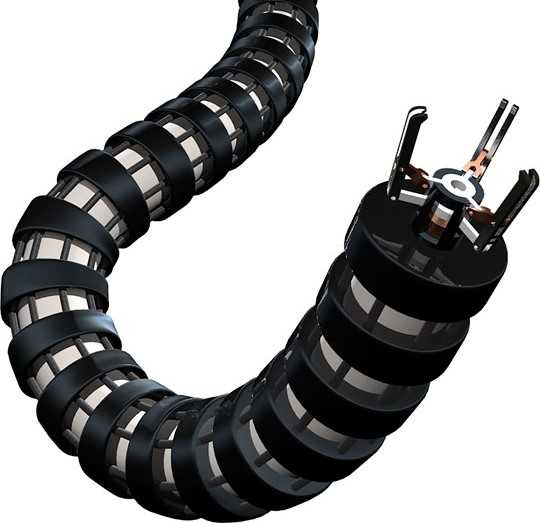
\includegraphics[width=.8\textwidth]{Image/LR/CR_example.jpg} 
%     \caption[An example of continuum robot]
%     {\centering \textit{\textbf{An example of continuum robot }}\cite{CR_example}.}
%     \label{fig:CR_example}
% \end{figure}
% \noindent Different types of continuum robots have different backbones, actuating and flexible components, but they are generally all 
% work under the same working principle stated above. \\
%%% METHODOLOGY %%%
\subsection{Methodology}
\subsubsection{Forward Kinematics} % Done by Zehao Ye
To derive the workspace of the manipulator for further analysis, the forward kinematics algorithm of the manipulator 
need to be conducted. The forward kinematics algorithm of the fishbone continuum robot\cite{fishboneCR} with one 
segment is given. However, utilizing this algorithm for calculation becomes complex while there are four modules in 
the manipulator. Additionally, the inverse kinematics algorithm also requires the assistance of forward kinematics 
algorithm for subsequent calculations using the composite coordinate transformation formula. Therefore, The relevant 
forward kinematics algorithm for subsequent calculations need to be derived. \\
The base coordinate system can be established with the centroid of base connector upper surface serving as the origin. 
The x-axis of the coordinate system is parallel to the backbone of Module 1, which is Module (2,2). Consequently, 
the backbones of Modules 1 and 3, which are Modules (2,2) and (2,1) are parallel to the x-axis of base coordinate 
system, while the backbones of Modules 2 and 4, which are Modules (1,2) and (1,1) are parallel to the y-axis of base 
coordinate system. The positions of the five centroids in the base coordinate system when the manipulator is in the 
initial posture are shown in Figure \ref{fig:kinematics model 0_0_0_0}. The upper surface centroids of the connectors 
are designated as $node_1$, $node_2$, $node_3$, $node_4$, and $node_5$. \\
\begin{figure}[H] %[H] "corresponds to start the figure Here" 
    \centering %alignment can be flushleft or flushright
    \captionsetup{labelsep=colon}
    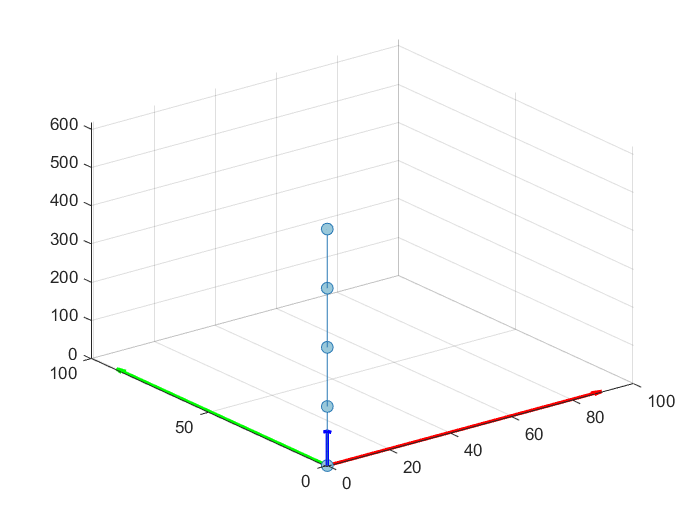
\includegraphics[width=1.0\textwidth]{Image/MATLAB/manipulator_0_0_0_0.png} 
    \caption[The kinematics model of manipulator in the initial position]
    {\centering \textbf{The kinematics model of manipulator in initial position.}}
    \label{fig:kinematics model 0_0_0_0}
\end{figure}
\noindent The Module 1 is restricted to bending in the y-z plane of the coordinate system where $node_1$ serves as 
the origin, while the Module 2 is restricted to bending in the x-z plane of the coordinate system where $node_2$ 
serves as the origin. Similarly, the Modules 3 and 4 are subject to the same constraints. The bending angles for 
these modules are defined as $\alpha_1$, $\alpha_2$, $\alpha_3$, and $\alpha_4$, respectively. The positions of the 
manipulator model in the base coordinate system after bending each module by $90 \degree$ are illustrated in Figure 
\ref{fig:kinematics_model_resp}.
\begin{figure}[H] %[H] "corresponds to start the figure Here" 
    \centering %alignment can be flushleft or flushright
    \captionsetup{labelsep=colon}
    \begin{subfigure}{0.48\textwidth} % subfigure 1
        \centering
        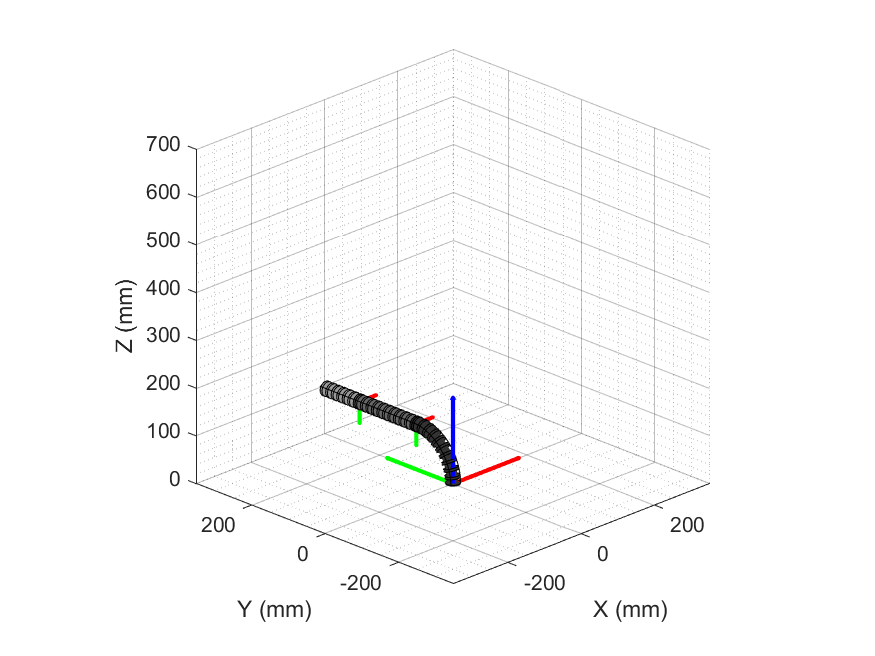
\includegraphics[width=\linewidth]{Image/MATLAB/manipulator_90_0_0_0.png}
        \caption{$\alpha_1=90 \degree,\alpha_2=0,\alpha_3=0,\alpha_4=0$}
    \end{subfigure}
    \hfill
    \begin{subfigure}{0.48\textwidth} % subfigure 2
        \centering
        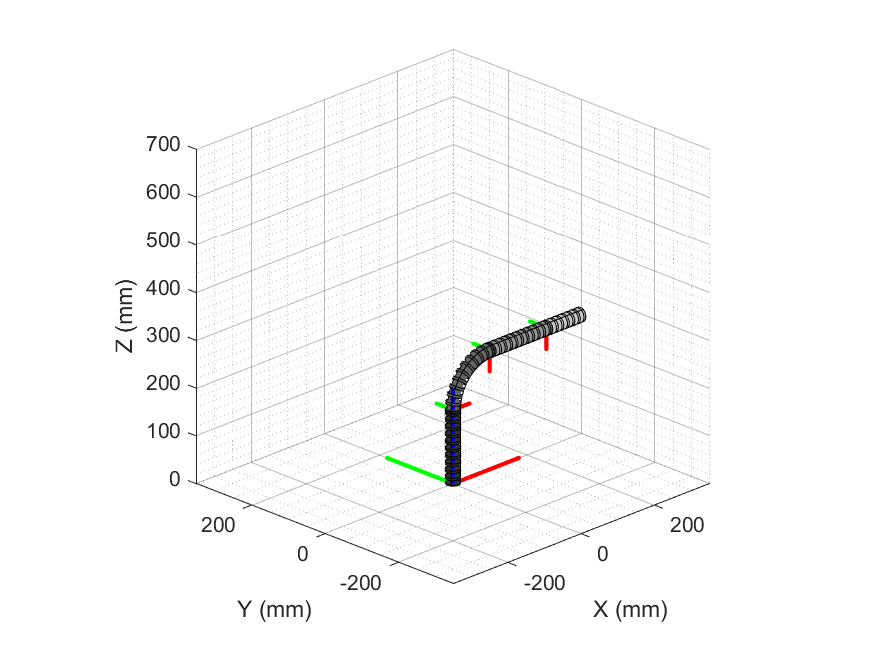
\includegraphics[width=\linewidth]{Image/MATLAB/manipulator_0_90_0_0.png}
        \caption{$\alpha_1=0,\alpha_2=90 \degree,\alpha_3=0,\alpha_4=0$}
    \end{subfigure}
    \begin{subfigure}{0.48\textwidth} % subfigure 3
        \centering
        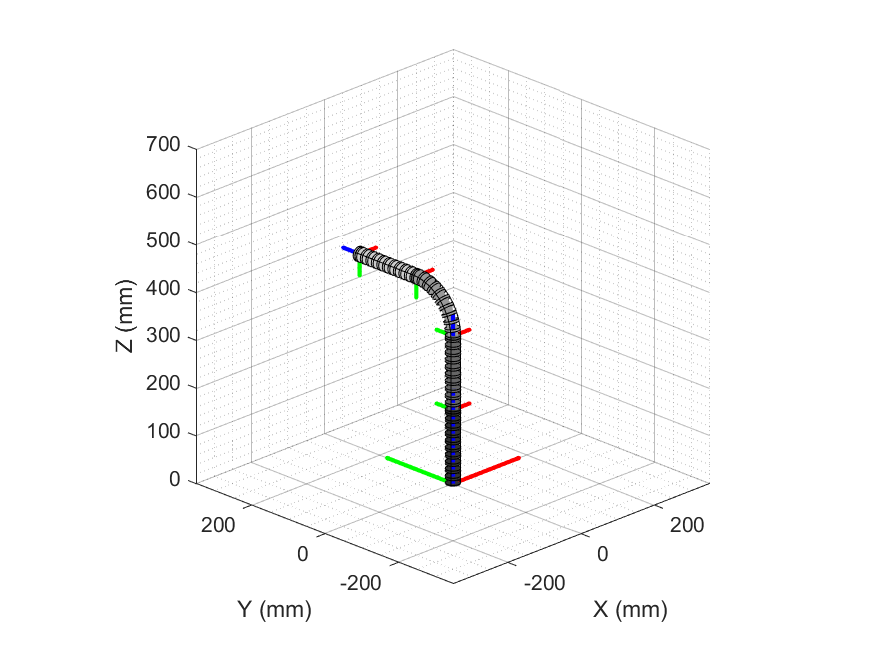
\includegraphics[width=\linewidth]{Image/MATLAB/manipulator_0_0_90_0.png}
        \caption{$\alpha_1=0,\alpha_2=0,\alpha_3=90 \degree,\alpha_4=0$}
    \end{subfigure}
    \hfill
    \begin{subfigure}{0.48\textwidth}
        \centering
        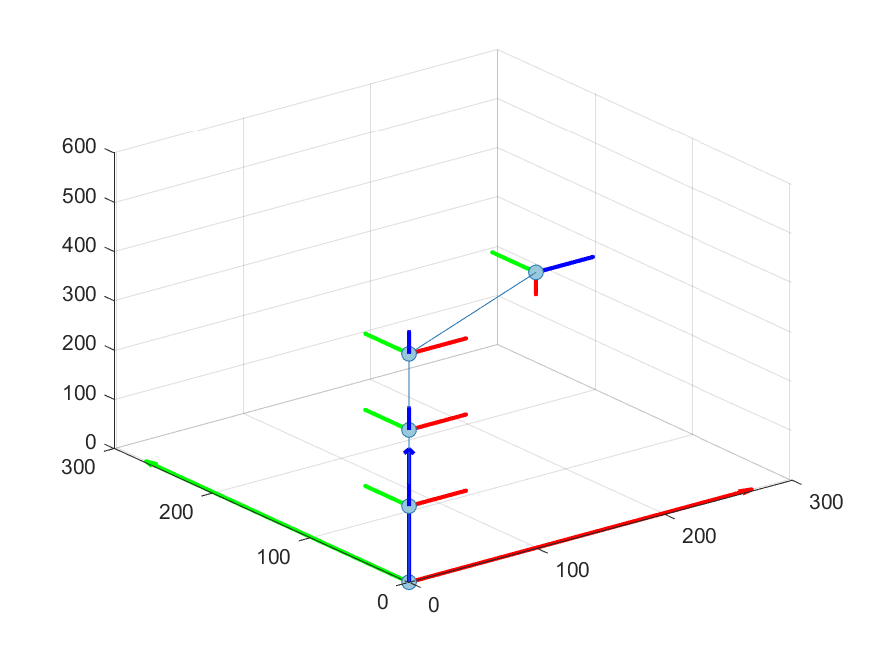
\includegraphics[width=\linewidth]{Image/MATLAB/manipulator_0_0_0_90.png}
        \caption{$\alpha_1=0,\alpha_2=0,\alpha_3=0,\alpha_4=90 \degree$}
    \end{subfigure}
    \caption[The kinematics model of manipulator with respective bending modules]
    {\centering \textbf{The kinematics model of manipulator with respective bending modules.}}
    \label{fig:kinematics_model_resp}
\end{figure}
\noindent While the modules bend to the positive direction of x-axis or y-axis, the bending angles $\alpha$ are 
positive. Owing to the distinct properties of the four modules, different calculation methods are required for analysis. 
The Module $i$ have a base node $node_i$ and an end effector node $node_{i+1}$. To further calculate the position of 
$node_{i+1}$ in the base coordinate system, these matrices can be employed in the Equation \ref{eq:node i+1 calculation}.
\begin{align}
    &\textbf{P}_{i+1}^{base} = \textbf{R}_{i} \times \textbf{P}_{i+1}^{i} + \textbf{P}_{i}^{base}
    \label{eq:node i+1 calculation}
\end{align}
\begin{align*}
    &\ \textbf{P}_{i+1}^{base}\text{: The position of $node_{i+1}$ in the base coordinate system.}\\
    &\ \textbf{R}_{i}\text{: The rotational matrix tranforms the base coordinate system into coordinate}\\
    &\ \qquad\text{system \textit{i}, which is the coordinate system with origin $node_i$.}\\
    &\ \textbf{P}_{i+1}^{i}\text{: The position of $node_{i+1}$ in coordinate system \textit{i}.}\\
    &\ \textbf{P}_{i}^{base}\text{: The position of $node_{i}$ in the base coordinate system.}
\end{align*}
\begin{itemize}
    \item Module 1 \\
    For Module 1, the relative position matrix of $node_1$ and $node_2$ $\textbf{P}_{2}^{1}$ and $\alpha_1$ is shown 
    in Equation \ref{eq:node2_postion_relative}. $R_1$ is the radius of the Module 1 bending curve. The rotational 
    matrix $\textbf{R}_{1}$ and the position matrix of $node_1$ $\textbf{P}_{1}^{base}$ are shown in Equations 
    \ref*{eq:module1_rotation_matrix} and \ref{eq:node1_position_absolute}.
    \begin{align}
        \textbf{P}_{2}^{1} = 
        \begin{bmatrix}
            0 \\
            (R_1\cdot(1-\cos(\alpha_1)) + d_2\cdot \sin(\alpha_1)) \\
            (R_1\cdot \sin(\alpha_1) + d_2\cdot \cos(\alpha_1)) \\
        \end{bmatrix}&
        \label{eq:node2_postion_relative} \\
        \nonumber (hint: \ R_1 = {Sr}_1/ &\alpha_1)
    \end{align}
    \vspace{-15mm}
    \begin{align}
        &\begin{aligned}
            \textbf{R}_{1} = 
            \begin{bmatrix}
                1 & 0 & 0 \\
                0 & 1 & 0 \\
                0 & 0 & 1 \\
            \end{bmatrix}
        \end{aligned}
        \label{eq:module1_rotation_matrix} \\
        &\begin{aligned}
            \textbf{P}_{1}^{base} = 
            \begin{bmatrix}
                0 & 0 & 0\\
            \end{bmatrix}^{\textbf{T}}
        \end{aligned}
        \label{eq:node1_position_absolute}
    \end{align}
    According to the Equations \ref{eq:node2_postion_relative}, \ref*{eq:module1_rotation_matrix}, and 
    \ref{eq:node1_position_absolute}, the position matrix of $node_{2}$ in the base coordinate system 
    $\textbf{P}_{2}^{base}$ can be calculated in Equation \ref{eq:node2_position_absolute}.
    \begin{align}
        &\textbf{P}_{2}^{base} = \textbf{R}_{1} \times \textbf{P}_{2}^{1} + \textbf{P}_{1}^{base} \nonumber \\
        &=
        \begin{bmatrix}
            1 & 0 & 0 \\
            0 & 1 & 0 \\
            0 & 0 & 1 \\
        \end{bmatrix}
        \times
        \begin{bmatrix}
            0 \\
            (R_1\cdot(1-\cos(\alpha_1)) + d_2\cdot \sin(\alpha_1)) \\
            (R_1\cdot \sin(\alpha_1) + d_2\cdot \cos(\alpha_1)) \\
        \end{bmatrix}
        +
        \begin{bmatrix}
            0 \\
            0 \\
            0 \\
        \end{bmatrix} \nonumber \\
        &=
        \begin{bmatrix}
            0 \\
            (R_1\cdot(1-\cos(\alpha_1)) + d_2\cdot \sin(\alpha_1)) \\
            (R_1\cdot \sin(\alpha_1) + d_2\cdot \cos(\alpha_1)) \\
        \end{bmatrix}
        \label{eq:node2_position_absolute}
    \end{align}
    \item Module 2 \\
    For Module 2, the relationship between the relative position matrix of $node_2$ and $node_3$ $\textbf{P}_{3}^{2}$ 
    and $\alpha_2$ is shown in Equation \ref{eq:node3_postion_relative}. $R_2$ is the radius of the Module 2 bending 
    curve. The rotational matrix $\textbf{R}_{2}$ and the position matrix of $node_2$ $\textbf{P}_{2}^{base}$ are shown 
    in Equations \ref*{eq:module2_rotation_matrix} and \ref{eq:node2_position_absolute}.
    \begin{align}
        \textbf{P}_{3}^{2} = 
        \begin{bmatrix}
            (R_2\cdot(1-\cos(\alpha_2)) + d_3\cdot \sin(\alpha_2)) \\
            0 \\
            (R_2\cdot \sin(\alpha_2) + d_3\cdot \cos(\alpha_2)) \\
        \end{bmatrix}&
        \label{eq:node3_postion_relative} \\
        \nonumber (hint: \ R_2 = {Sr}_2/ &\alpha_2)
    \end{align}
    \vspace{-15mm}
    \begin{align}
        &\begin{aligned}
            \textbf{R}_{2} = 
            \begin{bmatrix}
                1 & 0 & 0 \\
                0 & \cos(\alpha_1) & \sin(\alpha_1) \\
                0 & -\sin(\alpha_1) & \cos(\alpha_1) \\
            \end{bmatrix}
        \end{aligned}
        \label{eq:module2_rotation_matrix}
    \end{align}
    According to the Equations \ref{eq:node2_position_absolute}, \ref{eq:node3_postion_relative}, and 
    \ref*{eq:module2_rotation_matrix},     the position matrix of $node_{3}$ in the base coordinate system 
    $\textbf{P}_{3}^{base}$ can be calculated in Equation \ref{eq:node3_position_absolute}.
    \begin{align}
        &\textbf{P}_{3}^{base} = \textbf{R}_{1} \times \textbf{R}_{2} \times \textbf{P}_{3}^{2} + \textbf{P}_{2}^{base} \nonumber \\
        &= 
        \begin{bmatrix}
            1 & 0 & 0 \\
            0 & 1 & 0 \\
            0 & 0 & 1 \\
        \end{bmatrix}
        \times
        \begin{bmatrix}
            1 & 0 & 0 \\
            0 & \cos(\alpha_1) & \sin(\alpha_1) \\
            0 & -\sin(\alpha_1) & \cos(\alpha_1) \\
        \end{bmatrix} \nonumber \\
        &\times
        \begin{bmatrix}
            (R_2\cdot(1-\cos(\alpha_2)) + d_3\cdot \sin(\alpha_2)) \\
            0 \\
            (R_2\cdot \sin(\alpha_2) + d_3\cdot \cos(\alpha_2)) \\
        \end{bmatrix} \nonumber \\
        &+
        \begin{bmatrix}
            0 \\
            (R_1\cdot(1-\cos(\alpha_1)) + d_2\cdot \sin(\alpha_1)) \\
            (R_1\cdot \sin(\alpha_1) + d_2\cdot \cos(\alpha_1)) \\
        \end{bmatrix}
        \label{eq:node3_position_absolute}
    \end{align}
    \item Module 3 \\
    For Module 3, the relationship between the relative position matrix of $node_3$ and $node_4$ $\textbf{P}_{4}^{3}$ 
    and $\alpha_3$ is shown in Equation \ref{eq:node4_postion_relative}. $R_3$ is the radius of the Module 3 bending 
    curve. The rotational matrix $\textbf{R}_{3}$ and the position matrix of $node_3$ $\textbf{P}_{3}^{base}$ are shown 
    in Equations \ref*{eq:module3_rotation_matrix} and \ref{eq:node3_position_absolute}.
    \begin{align}
        \textbf{P}_{4}^{3} = 
        \begin{bmatrix}
            0 \\
            (R_3\cdot(1-\cos(\alpha_3)) + d_4\cdot \sin(\alpha_3)) \\
            (R_3\cdot \sin(\alpha_3) + d_4\cdot \cos(\alpha_3)) \\
        \end{bmatrix}&
        \label{eq:node4_postion_relative} \\
        \nonumber (hint: \ R_2 = {Sr}_2/ &\alpha_2)
    \end{align}
    \vspace{-15mm}
    \begin{align}
        &\begin{aligned}
            \textbf{R}_{3} = 
            \begin{bmatrix}
                \cos(\alpha_2) & 0 & \sin(\alpha_2) \\
                0 & 1 & 0 \\
                -\sin(\alpha_2) & 0 & \cos(\alpha_2) \\
            \end{bmatrix}
        \end{aligned}
        \label{eq:module3_rotation_matrix}
    \end{align}
    According to the Equations \ref{eq:node3_position_absolute}, \ref{eq:node4_postion_relative}, and 
    \ref*{eq:module3_rotation_matrix},     the position matrix of $node_{4}$ in the base coordinate system 
    $\textbf{P}_{4}^{base}$ can be calculated in Equation \ref{eq:node4_position_absolute}.
    \begin{align}
        &\textbf{P}_{4}^{base} = \textbf{R}_{1} \times\textbf{R}_{2} \times\textbf{R}_{3} \times \textbf{P}_{4}^{3} + \textbf{P}_{3}^{base} \nonumber \\
        &= \textbf{R}_{1}\times\textbf{R}_{2}\times
        \begin{bmatrix}
            \cos(\alpha_2) & 0 & \sin(\alpha_2) \\
            0 & 1 & 0 \\
            -\sin(\alpha_2) & 0 & \cos(\alpha_2) \\
        \end{bmatrix} \nonumber \\
        &\times
        \begin{bmatrix}
            0 \\
            (R_3\cdot(1-\cos(\alpha_3)) + d_4\cdot \sin(\alpha_3)) \\
            (R_3\cdot \sin(\alpha_3) + d_4\cdot \cos(\alpha_3)) \\
        \end{bmatrix} + \textbf{P}_{3}^{base}
        \label{eq:node4_position_absolute}
    \end{align}
    \item Module 4 \\
    In summary, the position matrix of $node_5$ in the base coordinate system $P_5^{base}$can be represented by 
    Equation \ref{eq:node5_position_absolute}.
    \begin{align}
        \textbf{P}_{5}^{base} = \textbf{R}_{1} \times\textbf{R}_{2} \times\textbf{R}_{3} \times\textbf{R}_{4} \times \textbf{P}_{5}^{4} + \textbf{P}_{4}^{base}
        \label{eq:node5_position_absolute}
    \end{align}
\end{itemize}
Applying the corresponding transformations to the Equation \ref{eq:node i+1 calculation} reveals the patterns shown 
in Equations \ref{eq:nodei+1_position_absolute_minus} and \ref{eq:nodei+1_position_absolute}.
\begin{align}
    &\textbf{P}_{i+1}^{base} - \textbf{P}_{i}^{base} = \prod_{n=1}^{i}\textbf{R}_{n}\times \textbf{P}_{i+1}^{i} 
    \label{eq:nodei+1_position_absolute_minus} \\
    &\textbf{P}_{i+1}^{base} = \sum_{m=1}^{i}\left[\prod_{n=1}^{m}\textbf{R}_{n}\times \textbf{P}_{m+1}^{m}\right] \quad(\textbf{P}_{1}^{base} = 0)
    \label{eq:nodei+1_position_absolute}
\end{align}
To emphasize transformation of manipulator, homogeneous transformation matrices \cite{homogeneous} are 
employed to describe the position of the end effector of the manipulator in Equations \ref{eq:homogeneous_matrix} 
and \ref{eq:homogeneous_matrices}.

\begin{align}
    &\textbf{H}_{i+1}^{i} = 
    \begin{bmatrix}
        \textbf{R}_{i+1}^{i} &  \textbf{P}_{i+1}^{i}\\
        0_{1\times3} & 1 \\
    \end{bmatrix} 
    \label{eq:homogeneous_matrix} \\
    &\begin{bmatrix}
        \textbf{P}_{i+1}^{base} \\
        1 \\
    \end{bmatrix}
    = \prod_{j=1}^{i}\textbf{H}_{j+1}^{j} \ 
    \times
    \begin{bmatrix}
        \textbf{P}_{i+1}^{i} \\
        1 \\
    \end{bmatrix} 
    \label{eq:homogeneous_matrices}
\end{align}

\subsubsection{Inverse Kinematics} % Done by Zehao Ye
The inverse kinematics algorithm is inspired by a rigid manipulator inverse kinematics solver called FABRIK 
\cite{fabrik}. W. Zhang et al.\cite{fabrikc} expanded this solver to the continuum manipulator domain. Considering 
the distinctive nature of the manipulator, adaptations have been implemented to the FABRIKc solver, transforming it 
into a tailored inverse kinematics algorithm for this particular application. For further elucidation, the inverse 
kinematics derivation is demostrated using the posture where $\alpha_1 = 0$, $\alpha_2 = 0$, $\alpha_1 = 90$, and 
$\alpha_4 = 0$. The comprehensive process of the first epoch will be elaborated. The iterative procedure of epoch 1 
is elucidated as follow. Simultaneously, the flowchart of FABRIKc algorithm is shown in Figure \ref{fig:flowchart}. \\
\begin{figure}[H]
    \centering
    \captionsetup{labelsep=colon}
    \begin{tikzpicture}[node distance=1.5cm,every node/.style={fill=white, font=\sffamily}, align=center]
        % Specification of nodes (position, etc.)
        \node (input) [data]   
        {\textbf{Input}: $\textbf{O}_{target}$, $\textbf{P}_{target}$, $\boldsymbol{\epsilon}$, ${epo}_{max}$ };
        \node (start) [activityStarts, below of=input] {Start};
        \node (init) [process, below of=start]          
        {Initialization: $\textbf{vnode}_i$, $\textbf{node}_i$, $\textbf{l}_i$};
        \node (value) [process, below of=init]   
        {epo = 1, $\textbf{e} = \lVert\textbf{P}_{target} - \textbf{P}_{\theta_1, \theta_2, \theta_3, \theta_4}\rVert$};
        \node (deter) [pending, below of=value, yshift=-15mm]   
        {$\textbf{e} > \boldsymbol{\epsilon}$ \&\& \\ $epo < {epo}_{max}$};
        \node (frp) [process, below of=deter, yshift=-22mm, fill=red!25] {FABRIKc: Forward Reaching Phase};
        \node (brp) [process, below of=frp, fill=red!25] {FABRIKc: Back Reaching Phase};
        \node (plus) [process, below of=brp] {epo = epo + 1};  
        \node (deter_epo) [pending, right of=deter, xshift=55mm] {$epo > {epo}_{max}$};  
        \node (fail) [data, above of=deter_epo, yshift=25mm] {\textbf{Output}: $\theta_i$ with min $\textbf{e}$};  
        \node (success) [data, below of=deter_epo, yshift=-25mm] {\textbf{Output}: $\theta_i$ with $\textbf{e}$ and $epo$}; 
        \node (deltaS) [data, below of=success, yshift=-10mm] {\textbf{Output}: $\Delta S$};  
        % Specification of lines between nodes specified above
        % with aditional nodes for description 
        \draw[->]  (input) -- (start);
        \draw[->]  (start) -- (init);
        \draw[->]  (init) -- (value);
        \draw[->]  (value) -- (deter);
        \draw[->]  (deter) -- node {Yes}(frp);
        \draw[->]  (frp) -- (brp);
        \draw[->]  (brp) -- (plus);
        \draw[->]  (plus) -- ++(-3.6,0) -- ++(0,6.7) -- (deter);
        \draw[->]  (deter) -- node {No}(deter_epo);
        \draw[->]  (deter_epo) -- node {Yes}(fail);
        \draw[->]  (deter_epo) -- node {No}(success);
        \draw[->]  (success) -- node {conversion}(deltaS);
        \draw[->]  (fail) -- ++(3.0,0) -- node {conversion} ++(0,-10.5) -- (deltaS);
    \end{tikzpicture}
    \caption[The flow chart of the FABRIKc algorithm]
    {\centering \textbf{The flow chart of the FABRIKc algorithm.}}
    \label{fig:flowchart}
\end{figure}
Pimarily, the position and orientation of end effector can be calculated by forward kinematics algorithm conducted 
in Equation \ref{eq:homogeneous_matrix}. The orientation and position matrices of the target are derived in Equation 
\ref{eq:target_homo}. These matrices are utilized as the input of the FABRIKc algorithm. The output of the algorithm 
is a series of bending angles $\theta_1$, $\theta_2$, $\theta_3$, and $\theta_4$.
\begin{align}
    \textbf{O}_{target} = 
    \begin{bmatrix}
        1 & 0 & 0 \\
        0 & 0 & -1 \\
        0 & 1 & 0 \\
    \end{bmatrix} 
    \qquad
    \textbf{P}_{target} = 
    \begin{bmatrix}
        0 \\
        245.493 \\
        395.493 \\
    \end{bmatrix} 
    \label{eq:target_homo} 
\end{align}
Additionally, it is essential to introduce a novel concept called "virtual node". This arised from the fact that FABRIK 
algorithm was originally designed for rigid manipulators, which implied that continuum manipulators need to be abstracted 
for modeling purpose. In this content, the module of manipulator are abstracted as a rigid manipulator with two prismatic 
joints and one revolute joint. The location of the revolute joint serves as the virtual node. \\
Subsequently, the forward reaching phase of the FABRIKc algorithm can commence. The calculation which involves four 
iterations is specified as follow.
\begin{itemize}
    \item Initialization \\
    The manipulator is estimated to stay at the initial position, which is shown in Figure 
    \ref{fig:kinematics model 0_0_0_0}. Under this circumstance, the nodes and virtual nodes of the manipulator 
    $\textbf{node}_{i}$ and $\textbf{vnode}_{i}$ are listed in Equations \ref{eq:node_initial} and 
    \ref{eq:virtual_node_initial}. The connector thickness of manipulator are not taken into account in this 
    demonstration, despite being considered in the programme. The virtual length $\textbf{l}_{i}$ for Module i, which 
    is the distance from $\textbf{vnode}_{i}$ to $\textbf{node}_{i}$ as well as ${node}_{i+1}$, is derived in Equation 
    \ref{eq:virtual_length}.
    \begin{align}
        & \textbf{node}_{1} = \begin{bmatrix} 0 \\ 0 \\ 0 \\ \end{bmatrix} 
        \textbf{node}_{2} = \begin{bmatrix} 0 \\ 0 \\ 150 \\ \end{bmatrix} 
        \textbf{node}_{3} = \begin{bmatrix} 0 \\ 0 \\ 300 \\ \end{bmatrix} 
        \textbf{node}_{4} = \begin{bmatrix} 0 \\ 0 \\ 450 \\ \end{bmatrix} 
        \textbf{node}_{5} = \begin{bmatrix} 0 \\ 0 \\ 600 \\ \end{bmatrix} 
        \label{eq:node_initial} \\
        &\textbf{vnode}_{1} = \begin{bmatrix} 0 \\ 0 \\ 75 \\ \end{bmatrix} 
        \textbf{vnode}_{2} = \begin{bmatrix} 0 \\ 0 \\ 225 \\ \end{bmatrix} 
        \textbf{vnode}_{3} = \begin{bmatrix} 0 \\ 0 \\ 375 \\ \end{bmatrix} 
        \textbf{vnode}_{4} = \begin{bmatrix} 0 \\ 0 \\ 525 \\ \end{bmatrix} 
        \label{eq:virtual_node_initial} 
    \end{align}
    \begin{align}
        &\textbf{l}_{i} = \frac{Sr_i}{\theta_i}\cdot \tan(\theta_i)
        \quad (hint: \ \textbf{l}_{i} = {Sr}_i/2 \ while \ \theta_i = 0) \label{eq:virtual_length}\\
        &\textbf{l}_{1} = \textbf{l}_{2} = \textbf{l}_{3} = \textbf{l}_{4} = 75 \ (unit: \ mm) \nonumber
    \end{align}
    \item Iteration 1 \\ % ITEM 1
    The virtual node of Module 4 can be derived by $\textbf{O}_{target}$ and $\textbf{P}_{target}$ in Equation 
    \ref{eq:target_homo}. The virtual node $\textbf{vnode}_{4}$ can be derived by Equation \ref{eq:vnode4_origin}.
    \begin{align}
        &\textbf{vnode}_{4}^{'} = \textbf{P}_{target} - \textbf{l}_{4} \cdot \textbf{O}_{target}^{z} \quad 
        (hint: \ ^{z} \ is \ z-axis \ orientation)
        \label{eq:vnode4_origin}
    \end{align}
    Afterwards, the vector from virtual node of Module 3 to virtual node of Module 4 can be derived based on the 
    positions of $\textbf{vnode}_{3}$ and $\textbf{vnode}_{4}^{'}$. The coordinate of the vector in the orientation 
    of $\textbf{vnode}_{4}^{'}$ can be calculated in Equation \ref{eq:vector_vn3tovn4}. 
    \begin{align}
        &\textbf{vector}_{4} = \textbf{O}_{target} \times (\textbf{vnode}_{4}^{'} - \textbf{vnode}_{3}) 
        \label{eq:vector_vn3tovn4} 
    \end{align}
    The bending angle of Module 4 $\theta_4$ can be derived in Equation \ref{eq:theta_4}. The y-axis directional 
    component is neglected because Module 4 can only bend in x-z plane. The updated length $\textbf{l}_{4}^{update}$ 
    can be calculated according to Equation \ref{eq:virtual_length_4}. Meanwhile, the updated 
    $\textbf{vnode}_{4}^{update}$ can be recalculated using $\textbf{l}_{4}^{update}$ in Equation \ref{eq:vnode4_update}. 
    The $\textbf{node}_4$ can also be determined based on the orientation of $\textbf{vnode}_{4}^{update}$, 
    which is $\textbf{O}_{vnode_4}$, in Equation \ref{eq:node4}.
    \begin{align}
        &\theta_4 = -arctan2(\textbf{vector}_{4}^{x},\textbf{vector}_{4}^{z})
        \label{eq:theta_4} \\
        &\textbf{l}_{4}^{update} = \frac{Sr_4}{\theta_4}\cdot \tan(\theta_4)
        \label{eq:virtual_length_4} \\
        &\textbf{vnode}_{4}^{update} = \textbf{P}_{target} - \textbf{l}_{4}^{update} \cdot \textbf{O}_{target}^{z}
        \label{eq:vnode4_update} \\
        &\textbf{O}_{vnode_4} =     
        \begin{bmatrix}
            cos(\theta_4) & 0 & sin(\theta_4) \\
            0 & 1 & 0 \\
            -sin(\theta_4) & 0 & sin(\theta_4) \\
        \end{bmatrix}  
        \times \textbf{O}_{target}
        \label{eq:orientation_vnode4} \\
        &\textbf{node}_4 = \textbf{vnode}_{4}^{update} - \textbf{l}_{4}^{update} \cdot \textbf{O}_{vnode_4}^{z}
        \label{eq:node4} 
    \end{align}
    \item Iteration 2 \\ % ITEM 2
    The virtual node of Module 3 can be derived by $\textbf{O}_{vnode_4}$ and $\textbf{node}_{4}$ in Equations 
    \ref{eq:orientation_vnode4} and \ref{eq:node4}. The virtual node $\textbf{vnode}_{3}$ can be derived by Equation 
    \ref{eq:vnode3_origin}.
    \begin{align}
        &\textbf{vnode}_{3}^{'} = \textbf{node}_{4} - \textbf{l}_{3} \cdot \textbf{O}_{vnode_4}^{z}
        \label{eq:vnode3_origin}
    \end{align}
    Afterwards, the vector from virtual node of Module 2 to virtual node of Module 3 can be derived based on the 
    positions of $\textbf{vnode}_{2}$ and $\textbf{vnode}_{3}^{'}$. The coordinate of the vector in the orientation 
    of $\textbf{vnode}_{3}^{'}$ can be calculated in Equation \ref{eq:vector_vn2tovn3}. 
    \begin{align}
        &\textbf{vector}_{3} = \textbf{O}_{vnode_3} \times (\textbf{vnode}_{3}^{'} - \textbf{vnode}_{2}) 
        \label{eq:vector_vn2tovn3} 
    \end{align}
    The bending angle of Module 3 $\theta_3$ can be derived in Equation \ref{eq:theta_3}. The x-axis directional 
    component is neglected because Module 3 can only bend in y-z plane. The updated length $\textbf{l}_{3}^{update}$ 
    can be calculated according to Equation \ref{eq:virtual_length_3}. Meanwhile, the updated 
    $\textbf{vnode}_{3}^{update}$ can be recalculated using $\textbf{l}_{3}^{update}$ in Equation \ref{eq:vnode3_update}. 
    The $\textbf{node}_3$ can also be determined based on the orientation of $\textbf{vnode}_{3}^{update}$, 
    which is $\textbf{O}_{vnode_3}$, in Equation \ref{eq:node3}.
    \begin{align}
        &\theta_3 = -arctan2(\textbf{vector}_{3}^{y},\textbf{vector}_{3}^{z})
        \label{eq:theta_3} \\
        &\textbf{l}_{3}^{update} = \frac{Sr_3}{\theta_3}\cdot \tan(\theta_3)
        \label{eq:virtual_length_3} \\
        &\textbf{vnode}_{3}^{update} = \textbf{node}_{4} - \textbf{l}_{3}^{update} \cdot \textbf{O}_{vnode_4}^{z}
        \label{eq:vnode3_update} \\
        &\textbf{O}_{vnode_3} =     
        \begin{bmatrix}
            1 & 0 & 0 \\
            0 & cos(\theta_3) & sin(\theta_3) \\
            0 & -sin(\theta_3) & sin(\theta_3) \\
        \end{bmatrix}  
        \times \textbf{O}_{vnode_4}
        \label{eq:orientation_vnode3} \\
        &\textbf{node}_3 = \textbf{vnode}_{3}^{update} - \textbf{l}_{3}^{update} \cdot \textbf{O}_{vnode_3}^{z}
        \label{eq:node3} 
    \end{align}
    \item Iteration 3 \\ % ITEM 3
    The virtual node of Module 2 can be derived by $\textbf{O}_{vnode_3}$ and $\textbf{node}_{3}$ in Equations 
    \ref{eq:orientation_vnode3} and \ref{eq:node3}. The virtual node $\textbf{vnode}_{2}$ can be derived by Equation 
    \ref{eq:vnode2_origin}.
    \begin{align}
        &\textbf{vnode}_{2}^{'} = \textbf{node}_{3} - \textbf{l}_{2} \cdot \textbf{O}_{vnode_3}^{z}
        \label{eq:vnode2_origin}
    \end{align}
    Afterwards, the vector from virtual node of Module 1 to virtual node of Module 2 can be derived based on the 
    positions of $\textbf{vnode}_{1}$ and $\textbf{vnode}_{2}^{'}$. The coordinate of the vector in the orientation 
    of $\textbf{vnode}_{2}^{'}$ can be calculated in Equation \ref{eq:vector_vn1tovn2}. 
    \begin{align}
        &\textbf{vector}_{2} = \textbf{O}_{vnode_2} \times (\textbf{vnode}_{2}^{'} - \textbf{vnode}_{1}) 
        \label{eq:vector_vn1tovn2} 
    \end{align}
    The bending angle of Module 2 $\theta_2$ can be derived in Equation \ref{eq:theta_2}. The y-axis directional 
    component is neglected because Module 2 can only bend in x-z plane. The updated length $\textbf{l}_{2}^{update}$ 
    can be calculated according to Equation \ref{eq:virtual_length_2}. Meanwhile, the updated 
    $\textbf{vnode}_{2}^{update}$ can be recalculated using $\textbf{l}_{2}^{update}$ in Equation \ref{eq:vnode2_update}. 
    The $\textbf{node}_2$ can also be determined based on the orientation of $\textbf{vnode}_{2}^{update}$, 
    which is $\textbf{O}_{vnode_2}$, in Equation \ref{eq:node2}.
    \begin{align}
        &\theta_2 = -arctan2(\textbf{vector}_{2}^{x},\textbf{vector}_{2}^{z})
        \label{eq:theta_2} \\
        &\textbf{l}_{2}^{update} = \frac{Sr_2}{\theta_2}\cdot \tan(\theta_2)
        \label{eq:virtual_length_2} \\
        &\textbf{vnode}_{2}^{update} = \textbf{node}_{3} - \textbf{l}_{2}^{update} \cdot \textbf{O}_{vnode_3}^{z}
        \label{eq:vnode2_update} \\
        &\textbf{O}_{vnode_2} =     
        \begin{bmatrix}
            cos(\theta_2) & 0 & sin(\theta_2) \\
            0 & 1 & 0 \\
            -sin(\theta_2) & 0 & sin(\theta_2) \\
        \end{bmatrix}  
        \times \textbf{O}_{vnode_3}
        \label{eq:orientation_vnode2} \\
        &\textbf{node}_2 = \textbf{vnode}_{2}^{update} - \textbf{l}_{2}^{update} \cdot \textbf{O}_{vnode_2}^{z}
        \label{eq:node2} 
    \end{align}
    \item Iteration 4 \\ % ITEM 4
    The virtual node of Module 1 can be derived by $\textbf{O}_{vnode_2}$ and $\textbf{node}_{2}$ in Equations 
    \ref{eq:orientation_vnode2} and \ref{eq:node2}. The virtual node $\textbf{vnode}_{1}$ can be derived by Equation 
    \ref{eq:vnode1_origin}.
    \begin{align}
        &\textbf{vnode}_{1}^{'} = \textbf{node}_{2} - \textbf{l}_{1} \cdot \textbf{O}_{vnode_2}^{z}
        \label{eq:vnode1_origin}
    \end{align}
    Afterwards, the coordinate of the vector in the orientation of $\textbf{vnode}_{1}^{'}$ can be directly calculated 
    in Equation \ref{eq:vector_n1tovn1}. This is because the $\textbf{O}_{node_1}^{z}$ must be oriented vertically upward.
    \begin{align}
        &\textbf{vector}_{2} = \textbf{O}_{vnode_1} \times \begin{bmatrix} 0 & 0 & 1 \end{bmatrix} 
        \label{eq:vector_n1tovn1} 
    \end{align}
    The bending angle of Module 1 $\theta_1$ can be derived in Equation \ref{eq:theta_1}. The x-axis directional 
    component is neglected because Module 1 can only bend in y-z plane. The updated length $\textbf{l}_{1}^{update}$ 
    can be calculated according to Equation \ref{eq:virtual_length_1}. Meanwhile, the updated 
    $\textbf{vnode}_{1}^{update}$ can be recalculated using $\textbf{l}_{1}^{update}$ in Equation \ref{eq:vnode1_update}. 
    The $\textbf{node}_1$ can also be determined based on the orientation of $\textbf{vnode}_{1}^{update}$, 
    which is $\textbf{O}_{vnode_1}$, in Equation \ref{eq:node1}.
    \begin{align}
        &\theta_1 = -arctan2(\textbf{vector}_{1}^{y},\textbf{vector}_{1}^{z})
        \label{eq:theta_1} \\
        &\textbf{l}_{1}^{update} = \frac{Sr_1}{\theta_1}\cdot \tan(\theta_1)
        \label{eq:virtual_length_1} \\
        &\textbf{vnode}_{1}^{update} = \textbf{node}_{2} - \textbf{l}_{1}^{update} \cdot \textbf{O}_{vnode_2}^{z}
        \label{eq:vnode1_update} \\
        &\textbf{O}_{vnode_1} =     
        \begin{bmatrix}
            1 & 0 & 0 \\
            0 & cos(\theta_1) & sin(\theta_1) \\
            0 & -sin(\theta_1) & sin(\theta_1) \\
        \end{bmatrix}  
        \times \textbf{O}_{vnode_2}
        \label{eq:orientation_vnode1} \\
        &\textbf{node}_1 = \textbf{vnode}_{1}^{update} - \textbf{l}_{1}^{update} \cdot \textbf{O}_{vnode_1}^{z}
        \label{eq:node1} 
    \end{align}
\end{itemize}
Ultimately, the FABRIKc algorithm initiates the backward reaching phase, which is forward kinematics algorithm. The 
FABRIKc algorithm inherently guarantees the orientation of manipulator end effector,  with the necessity to account 
solely for positional errors. The error can be calculated by Equation \ref{eq:error_calculation}.
\begin{align}
    \textbf{e} = \lVert\textbf{P}_{target} - \textbf{P}_{\theta_1, \theta_2, \theta_3, \theta_4}\rVert
    \label{eq:error_calculation}
\end{align}
For the first epoch, the results of FABRIKc algorithm are 
$\boldsymbol{\theta} = [6.71,\ -0.0,\ 83.29,\ -0.0]\degree $, 
The error of the first epoch is 33.77506. The results about FABRIKc algorithm with the target angle 
$\boldsymbol{\alpha} = [0,\ 0,\ 90,\ 0] $ are shown in Table \ref{tab:fabrikc_0_0_90_0} 
in Appendix \ref{append:table}. The algorithm has been configured to execute a maximum of 200 epochs, with 
the provision to pause when the error reaches a sufficiently low level, thereby conserving computational resources. 
The maximum epoch number is defined as ${epo}_{max}$. The error margin is $\boldsymbol{\epsilon}$.

\subsection{Electronic Control}
\subsubsection{Manipulator Actuation Control}
As mentioned above, the manipulator is divided into four units in total, with each unit being controlled for its 
bending movements by two cables. This means that the entire manipulator is controlled by a total of 8 cables. How 
to control the extension and retraction of these 8 cable ropes is the key to the Control part. \\
In this project, 8 stepper motors are employed to control the 8 individual cables. The planned design involves 
wrapping the cables around the rotor of each motor, and the stepper motors are programmed to extend or retract 
the ropes by stepping a certain number of steps in either a counterclockwise or clockwise direction. These 8 motors 
are connected to an Arduino board together, and the user can control the program by a keyboard, and a serial monitor. \\
\begin{itemize}
    \item Actuation Principle\\
    In this program, the user inputs the desired length changes for 8 cables $\Delta S_1$ ~ $\Delta S_8$ 
    ($\Delta S_{1,2,3,4}$ ranging from -36.65mm to 36.65mm, $\Delta S_{5,6,7,8}$ ranging from -68.07 to 68.07mm). 
    After conversion, it outputs the corresponding step numbers $Step_1$ ~ $Step_8$ for the eight stepper motors. 
    Based on this, the 8-stepper motors will step the correspondingly. The relationship between the changes in 
    cable length and the motor steps can be defined by Equation \ref{eq:step_motor_arduino}. \\
    \begin{align}
        & \qquad\qquad\qquad\qquad Step_i=\frac{(\Delta S_i-\Delta S_{i(prev)})\cdot N}{\pi\cdot d}, \ i\in[1,8] 
        \label{eq:step_motor_arduino} \\
        &\Delta S_{i(prev)} \text{: The length change for $i^{th}$ cable in the previous location.} \nonumber \\
        &d\text{: The diameter of the rotor. A rotor of diameter 10mm is used currently.} \nonumber \\
        &N\text{: Number of steps/rev. 2048 for 28YBG-48 motor.}\nonumber 
    \end{align}
    \item Component Selection \\
    To achieve a successful and precise control functionality, the first thing to do is to select appropriate 
    components. Below are the main electronic components chosen:
    \begin{itemize}
        \item Arduino Mega 2560 board: \\
        Because the project requires connecting 8 motors at the same time, the board should have more pins on the 
        board as well as stronger processing capabilities compared to ordinary boards. Therefore, the Arduino Mega 
        2560 has been selected. It boasts up to 54 I/O pins and a more powerful processor to allow for better 
        performance in multitasking operations \cite{arduino_guide}.
        \item 28YBJ-48 stepper motor: \\
        The 28YBJ-48 stepper motor is currently one of the most commonly used stepper motors on the market. It 
        operates in two modes: half-step and full-step, corresponding to 4096 steps/rev and 2048 steps/rev 
        respectively. This high-resolution configuration allows the manipulator to perform high-precision 
        operations. Additionally, at its rated voltage, it can provide a torque of up to 34Nm, which is more than 
        sufficient for pulling the cables of a lightweight mechanical arm.
        \item ULN 2003A motor control chip: \\
        The motor control chip acts as the brain of the motor, responsible for translating instructions from the 
        Arduino board into operations that the motor can execute. The ULN2003A chip is specifically matched with 
        the 28YBJ-48 motor, ensuring seamless coordination and operation between the chip and the motor. 
        \item 9V power supply: \\
        The rated operating voltage of the stepper motor is 5-12V. Here, a 9V power supply is chosen to allow 
        losses due to component resistance. 
    \end{itemize}
    \item Circuit Schematics \\
    The schematic of the overall circuit for the manipulator actuation control part is shown in Figure \ref{fig:motor_circuit_layout}.
    \begin{figure}[H] %[H] "corresponds to start the figure Here" 
        \centering %alignment can be flushleft or flushright
        \captionsetup{labelsep=colon}
        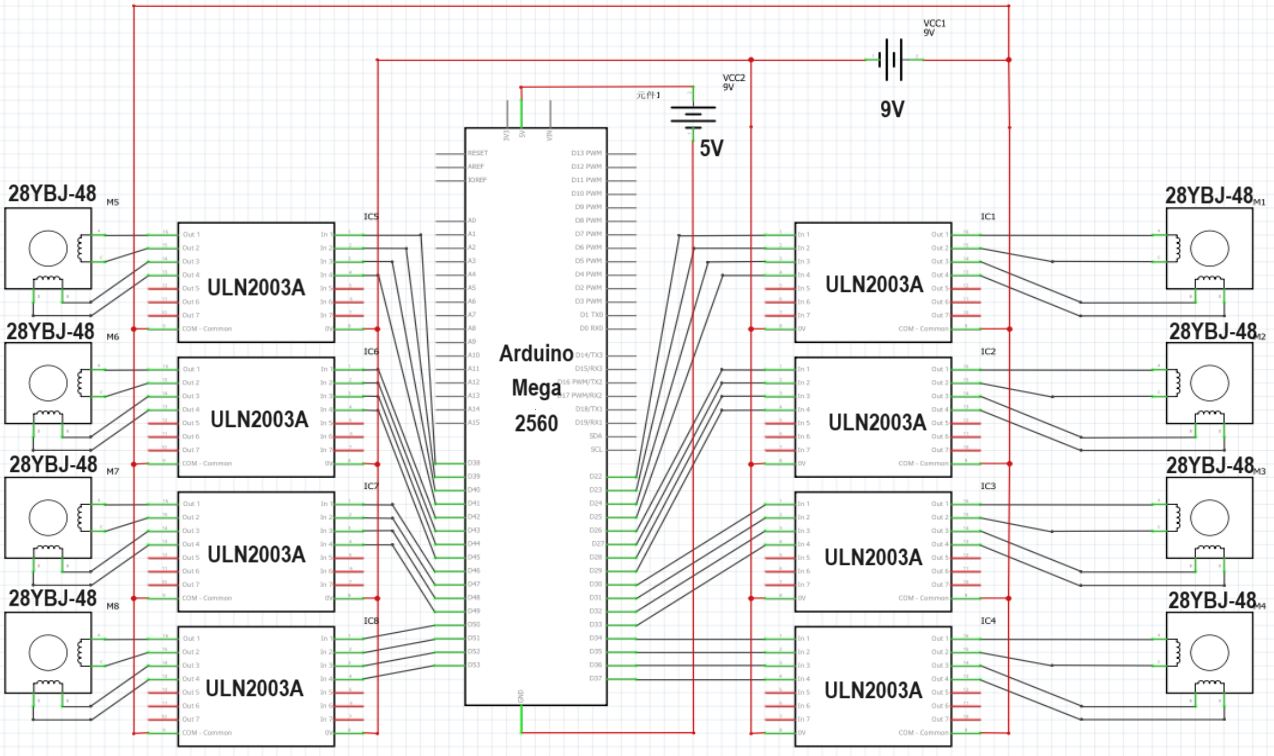
\includegraphics[width=0.7\textwidth]{Image/Design/arduino_circuit_layout.png} 
        \caption[The circuit layout of Arduino step motor control system]
        {\centering \textbf{The circuit layout of Arduino step motor control system.}}
        \label{fig:motor_circuit_layout}
    \end{figure}
    The 8 motors use pin 23-52 on the Arduino Mega 2560 board, and are powered by a 9V battery. The power supply 
    is in a parallel configuration on a breadboard. The Arduino board is connected to a serial monitor and a 
    keyboard for state inspection and manual input.
    \item Program development \\
    The main logic framework of the program has been illustrated by the flowchart shown in Figure \ref{fig:motor_flowchart}.
    \begin{figure}[H] %[H] "corresponds to start the figure Here" 
        \centering %alignment can be flushleft or flushright
        \captionsetup{labelsep=colon}
        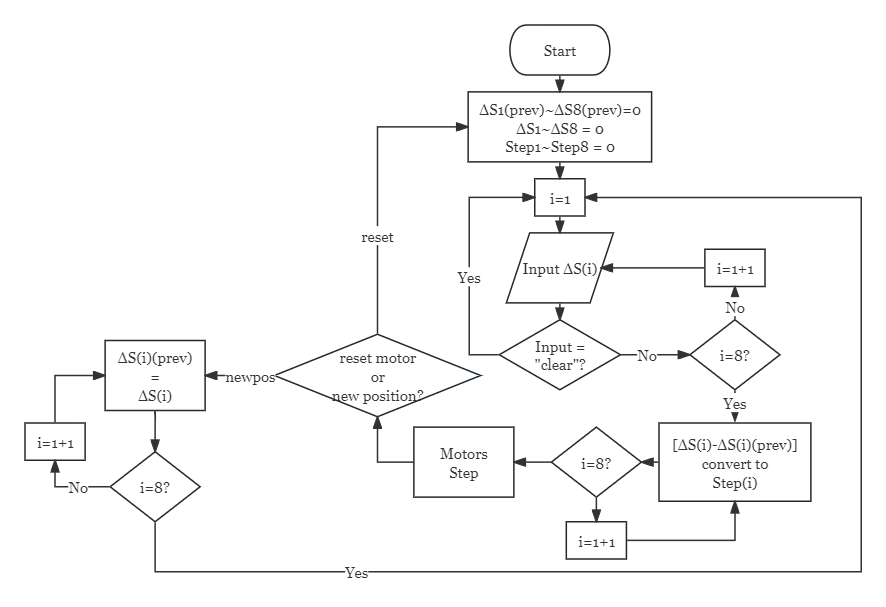
\includegraphics[width=1.0\textwidth]{Image/Design/flowchart_arduino_motor.png} 
        \caption[The flow chart of Arduino step motor control programme]
        {\centering \textbf{The flow chart of Arduino step motor control programme.}}
        \label{fig:motor_flowchart}
    \end{figure}
    After the program starts, the first thing is to declare the variables. $\Delta S_{i(prev)}$, $\Delta S_i$ and 
    $Step_i$ is all set to 0 initially. \\ Then the program asks the users to input 8 numbers representing the 
    length change for 8 cables. The 8 values will be assigned to variable $\Delta S_1$ ~ $\Delta S_8$ in order. 
    During the input process, the user can input `clear' instead of numbers to clear all the previous input and 
    start over again from $\Delta S_1$. \\
    Once the input process is complete, the program converts the $\Delta S_1$~$\Delta S_8$ to $Step_1$ ~ $Step_8$ 
    based on Equation \ref{eq:step_motor_arduino}, with the $d$ set to 10mm, N set to 2048 steps/rev. The motors 
    will start to step immediately after the conversion is finished. \\
    During the stepping process, the motors controlling the first and second unit (the first 4 motors) are set 
    to have a stepping speed of 300 steps/second, and the motors controlling the third and fourth unit 
    (the last 4 motors) are set to have $\frac{300}{17.5}\cdot(17.5+15)\approx 557$ steps/second. This is because 
    the moving speed for the last two units should be $\frac{17.5+15}{17.5}$ times faster than the first two units 
    so that the 4 units can finish moving approximately at the same time. \\
    The program shall wait until the motors finished stepping. Once the stepping process is finished, the program 
    asks the user what to do next: reset the motors to initial position or move from the current position to the 
    next position. If the user chooses to reset the motors, all of the motors rotate backwards for same steps. 
    However, If the user chooses to let the motors move to a new position, the values for current $\Delta S_1$ ~ 
    $\Delta S_8$ will be stored to variable $\Delta S_{1(prev)}$ ~ $\Delta S_{8(prev)}$. The program then asks for 
    a new set of $\Delta S_1$ ~ $\Delta S_8$, then calculate the new $Step_1$ ~$Step_8$. Hence, the loop of the 
    program is closed.
\end{itemize}
\subsubsection{Parameter input by Serial Monitor}
In the operating logic, the control parameters are inputted through the keyboard to control the motion of the 
multiple stepper motors. The basic function is to input the steps into the serial monitor through the keyboard 
of the host computer and the input string will be read by the microcontroller and converted into data, which are 
used as the number of steps of the stepper motor movement. For easy operation and display, the input parameters 
need to be displayed as text on the screen of the LCD IIC. LCD IIC will be in the form of a 2-line, 16-bit display 
to show more content. \\
Logic flowchart of the code to control the motor and LCD IIC by inputting parameters with the serial monitor of 
the host computer is shown in Figure \ref{fig:cl_input}.
\begin{figure}[H] %[H] "corresponds to start the figure Here" 
    \centering %alignment can be flushleft or flushright
    \captionsetup{labelsep=colon}
    \begin{subfigure}{0.45\textwidth} % subfigure 1
        \centering
        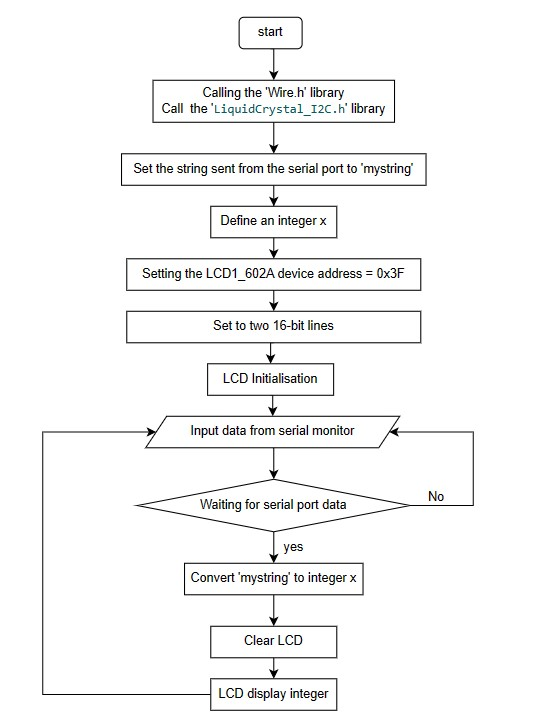
\includegraphics[width=\linewidth]{Image/Design/code_logic_input.jpg}
        \caption{\centering The code logic of using serial to input command parameter}
        \label{fig:cl_input}
    \end{subfigure}
    % \hfill
    \begin{subfigure}{0.45\textwidth} % subfigure 2
        \centering
        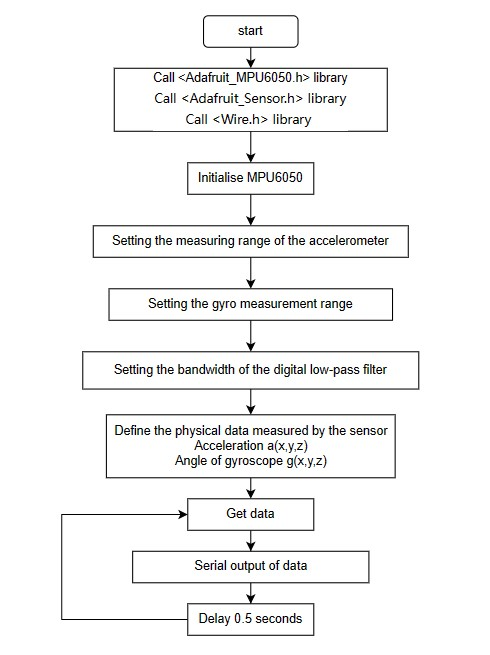
\includegraphics[width=\linewidth]{Image/Design/code_logic_angle.jpg}
        \caption{\centering The code logic of using MPU6050 to monitor gyro angles and accelerations}
        \label{fig:cl_angle}
    \end{subfigure}
    \caption[The code logic of input parameters and MPU6050]
    {\centering \textbf{The code logic of input parameters and MPU6050.}}
    \label{fig:cl_input_angle}
\end{figure}
\subsubsection{Verification of MPU 6050}
According to the project content, adding sensors to the end effector to measure its orientation angle and distance 
from the contact plane can assist the user to carry out more accurate operation. The function of detecting the 
orientation angle is realised by the MPU6050. \\
The Orientation angle (Euler angle) corresponding to the MPU6050 chip is shown in Figure \ref{fig:mpu6050_chip}. 
Pitch is rotation around the x-axis. Yaw is rotation around the y-axis. Roll is rotation around the z-axis. 
\begin{figure}[H] %[H] "corresponds to start the figure Here" 
    \centering %alignment can be flushleft or flushright
    \captionsetup{labelsep=colon}
    \begin{subfigure}{0.45\textwidth} % subfigure 1
        \centering
        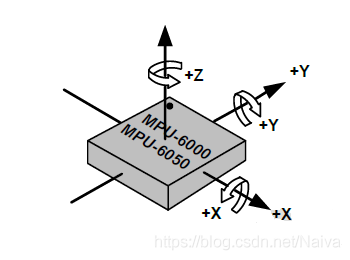
\includegraphics[width=\linewidth]{Image/Design/MPU6050_chip.png}
        \caption{\centering The MPU6050 chip corresponding to the Euler angle}
        \label{fig:mpu6050_chip}
    \end{subfigure}
    % \hfill
    \begin{subfigure}{0.45\textwidth} % subfigure 2
        \centering
        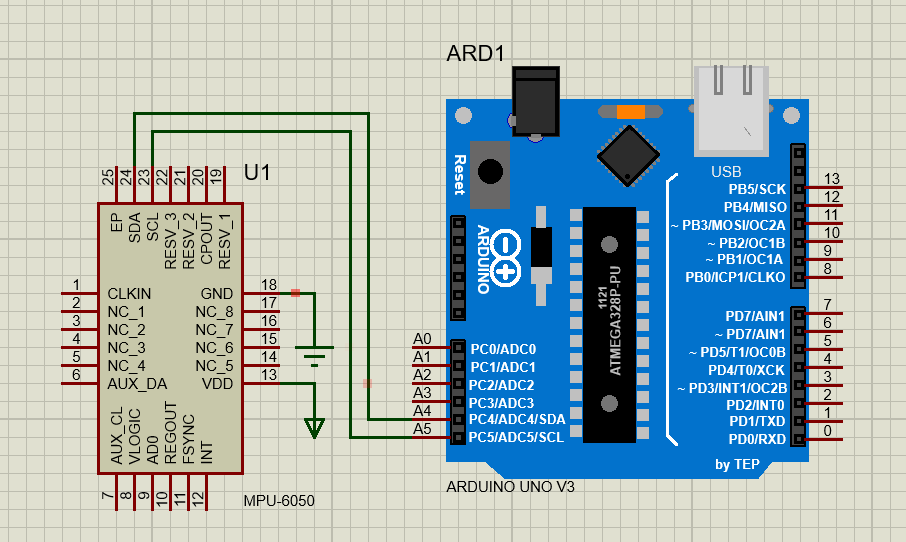
\includegraphics[width=\linewidth]{Image/Design/MPU6050_circuit.png}
        \caption{\centering The wiring diagram of MPU6050 and microcontroller}
        \label{fig:mpu6050_circuit}
    \end{subfigure}
    \caption[The MPU6050 chip with ancillary Arduino circuit]
    {\centering \textbf{The MPU6050 chip with ancillary Arduino circuit.}}
    \label{fig:mpu6050}
\end{figure}
\noindent The MPU6050 requires an external 5V power supply and GND. SCL is the Clock Pin of the IIC when the 
MPU6050 is used as a slave, and SDA is the Data Pin of the IIC when the MPU6050 is used as a slave. The wiring 
diagram is shown in Figure \ref{fig:mpu6050_circuit}. \\
The logic flowchart of the code that controls the MPU 6050 to display acceleration and direction angle is shown 
in Figure \ref{fig:cl_angle}. In this project, the acceleration parameters will not be acquired and displayed. \\
Since Proteus does not support dynamic simulation of the MPU6050, the verification of the MPU6050 has been 
carried out by physical parts and Arduino Mega while the project is in progress. The validation results have 
an acceptable accuracy and are able to display the corresponding orientation angle on the serial port and 
OLED screen. \\
\subsubsection{Using HC-SR04 to measure distance}
The HC-SR04 Ultrasonic Sensor uses sonar to determine the distance to an object. It has an ultrasonic 
transmitter and a receiver module which provides excellent non-contact range detection, high accuracy and 
stable readings. The measurement range is from 2 - 400 cm. The resolution is 0.3 cm and the measurement angle 
is within 30°. It operates in a process unaffected by sunlight or ferrous materials. \\
The sensor is triggered by sending a HIGH pulse of 10 microseconds. Previously, the speak gives a short 
low-level pulse to ensure that a clean HIGH pulse is obtained. \\
The basic principle of distance measurement is time of flight (Tof). The formula is as follows.
\begin{align}
    distance = (duration/2) \times v_{sound} \\
    v_{sound} = 343\ m/s = 1/29.1\ cm/us \nonumber
\end{align}
\noindent The wiring diagram and simulation results are shown in Figure \ref{fig:tof}. An SSD 1306 OLED screen 
is used to display the data in the simulation. The logic flowchart of the code that controls the HC-SR04 to measure 
distance and display acceleration by OLED screen is shown in Figure \ref{fig:cl_tof}.
\begin{figure}[H] %[H] "corresponds to start the figure Here" 
    \centering %alignment can be flushleft or flushright
    \captionsetup{labelsep=colon}
    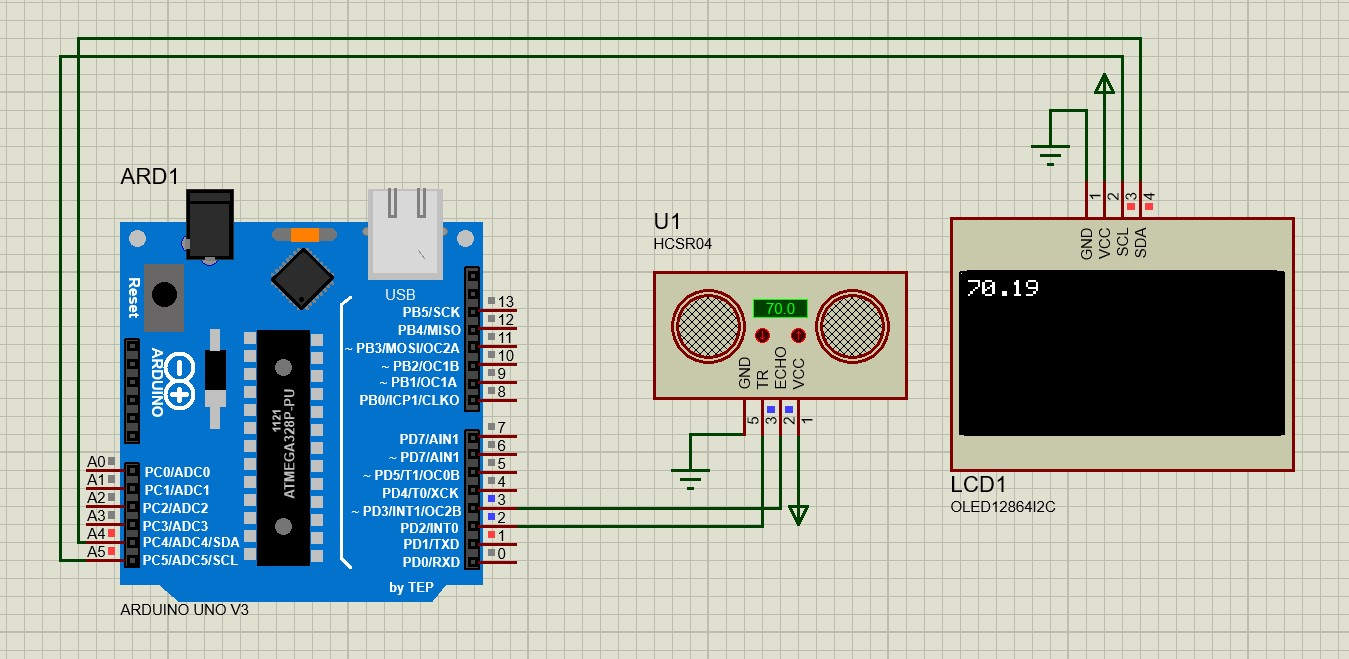
\includegraphics[width=0.8\linewidth]{Image/Design/tof_circuit.jpg}
    \caption[The wiring diagram and simulation of HC-SR04]
    {\centering \textbf{The wiring diagram and simulation of HC-SR04.}}
    \label{fig:tof}
\end{figure}
\begin{figure}[H] %[H] "corresponds to start the figure Here" 
    \centering %alignment can be flushleft or flushright
    \captionsetup{labelsep=colon}
    \begin{subfigure}{0.45\textwidth} % subfigure 1
        \centering
        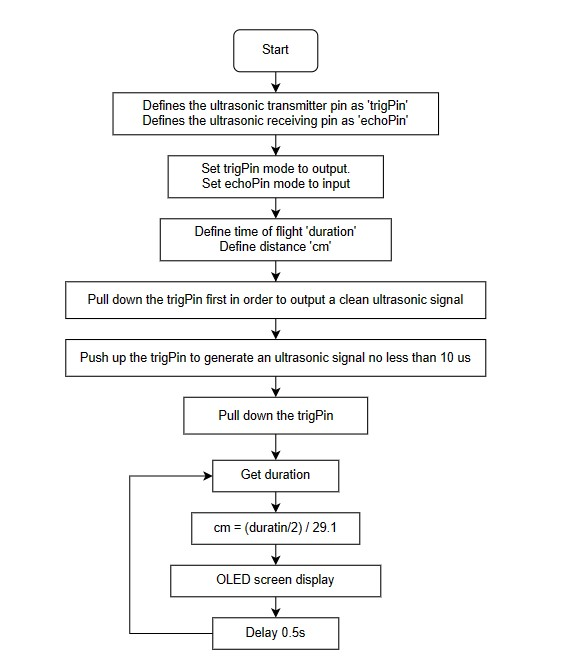
\includegraphics[width=\linewidth]{Image/Design/code_logic_tof.jpg}
        \caption{\centering The code logic of using HC-SR04 to measure distance}
        \label{fig:cl_tof}
    \end{subfigure}
    % \hfill
    \begin{subfigure}{0.45\textwidth} % subfigure 2
        \centering
        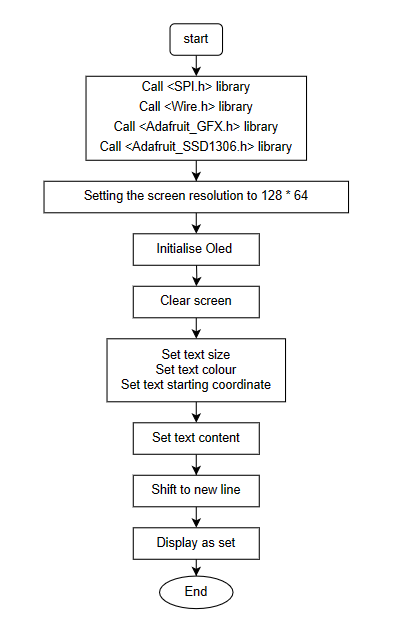
\includegraphics[width=\linewidth]{Image/Design/code_logic_display.png}
        \caption{\centering The code logic of using SSD 1306 OLED to display data}
        \label{fig:cl_oled}
    \end{subfigure}
    \caption[The code logic of HC-SR04 and SSD 1306 OLED]
    {\centering \textbf{The code logic of HC-SR04 and SSD 1306 OLED.}}
    \label{fig:cl_tof_oled}
\end{figure}
\subsubsection{SSD 1306 OLED}
Using SSD 1306 OLED requires calling two libraries, \lstinline{<Adafruit_SSD1306.h>} and 
\lstinline{<Adafruit_GFX.h>}. \lstinline{<Adafruit_SSD1306.h>} is a dedicated display library for SSD1306 OLED 
screens. \lstinline{<Adafruit_GFX.h>} library is the common parent graphics library for LCD and OLED screens. \\
The resolution of SSD1306 is 128x64 pixel dot array, SCK is the clock pin, SDA is the data pin, and external 
power supply and GND are required. Figure \ref{fig:cl_oled} is the logic flowchart of the code to control the 
OLED to display the text content.






% change to new page
\newpage 